\documentclass[12pt]{article}
\usepackage{amsmath}
\usepackage{amssymb}
\usepackage{graphicx}
\usepackage[margin=1in]{geometry}
\newcommand{\del}{\nabla}
\begin{document}

\title{Psych209 Final Project}
\author{Howon Lee}
\maketitle

%%%% to talk about

%explain the bak net
  How can you use extremal dynamics to train some kind of neural net?
  Qualitative model of evolution: Bak-Sneppen model.
  \begin{figure}
    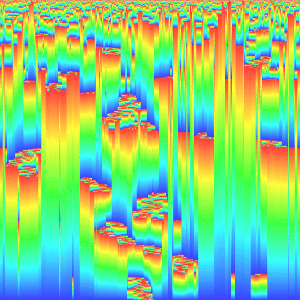
\includegraphics{bak_sneppen}
  \end{figure}

  Rules of Bak-Sneppen model. How does it behave? Criticality. Self-organized criticality.

  Caveats: CR Shalizi, W Tozier, "A Simple Model of the Evolution of Simple Models of Evolution"
  
  Bak and Chialvo's model

  More abstract: extremal optimization

  Finally: Using $\tau$-EO on RBM, classification results
  
  How it works, from 20000 feet
  \begin{figure}
    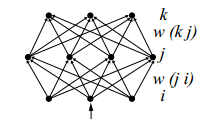
\includegraphics{bak_chialvo_net_topology}
  \end{figure}
  
  Problems: Conjunctive neurons
  \begin{figure}
    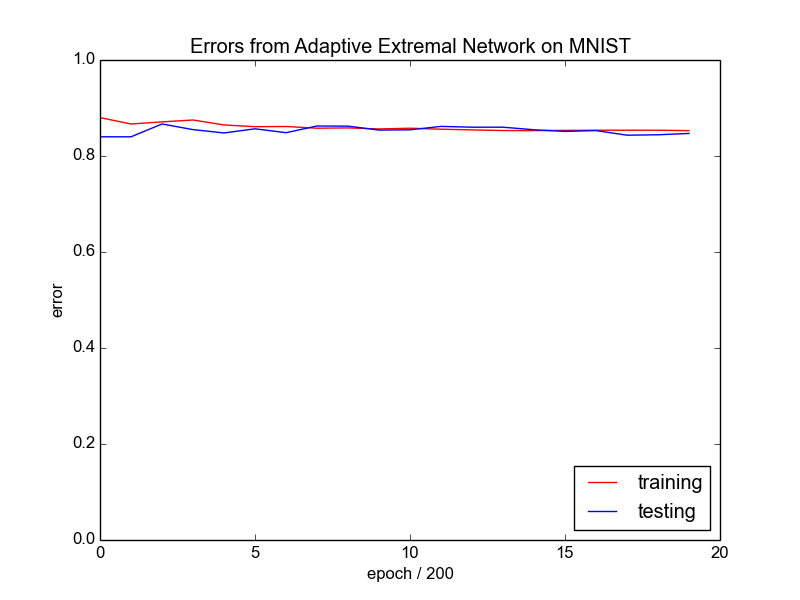
\includegraphics{bak_plot}
  \end{figure}

  Comparison to simulated annealing
  
  How it works, from 20000 feet

  Existing results, from Boetticher: TSP, Ising model

  $\tau$-EO
  
  \begin{figure}
    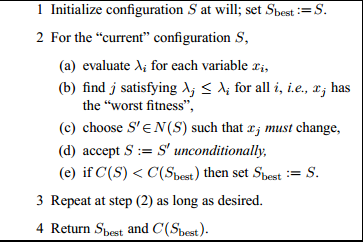
\includegraphics{eo_alg}
  \end{figure}
  
  The hope:
  \begin{figure}
    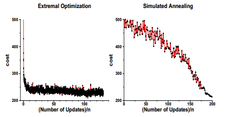
\includegraphics{boettcher}
  \end{figure}
  
  Why not feedforward? BM vs. Ising Model

  Locality: RBM

  \begin{figure}
    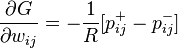
\includegraphics{rbm_eq}
  \end{figure}
  
  \frametitle{Ising Model}
  \begin{figure}
    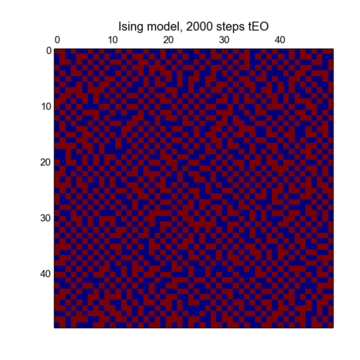
\includegraphics{2000}
  \end{figure}
  \begin{figure}
    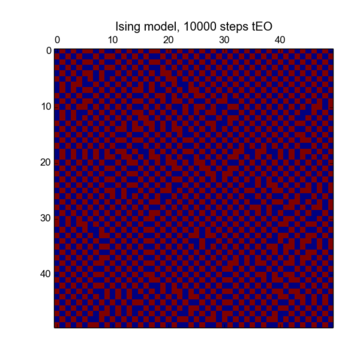
\includegraphics{10000}
  \end{figure}
  
  \frametitle{Ising Model}
  \begin{figure}
    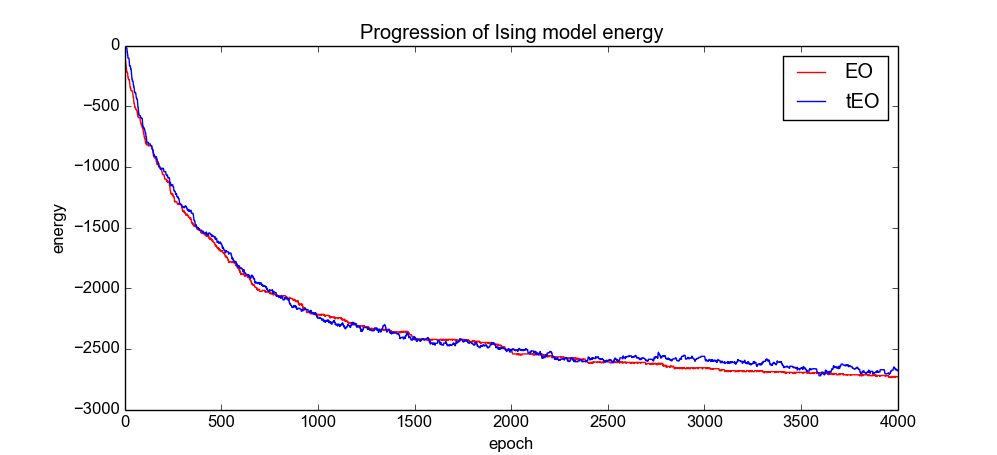
\includegraphics{ising_energy_unzoomed}
  \end{figure}
  
  \begin{figure}
    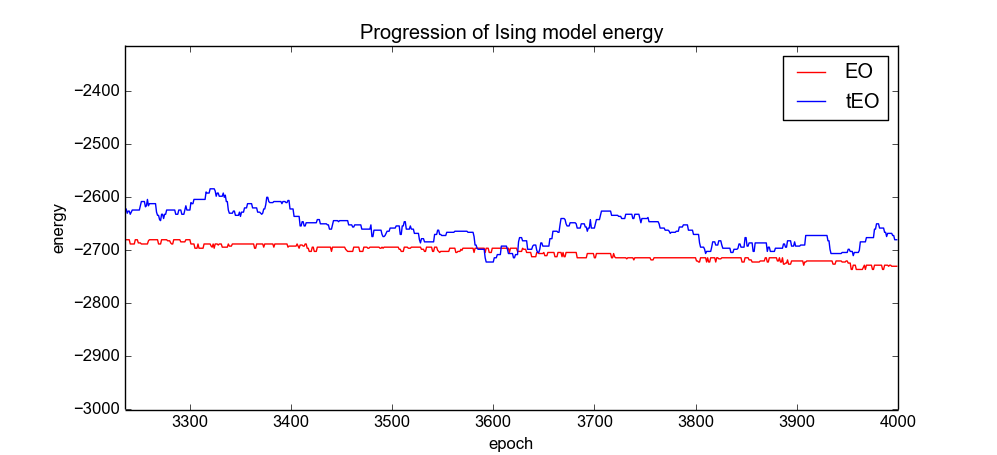
\includegraphics{ising_energy_zoomed}
  \end{figure}

  See performance in RBM learning, as simple as possible

  Bit string: metaphor of Hamming cliff in GA

  Actually, this is just a weird coordinate descent
  
  \begin{figure}
    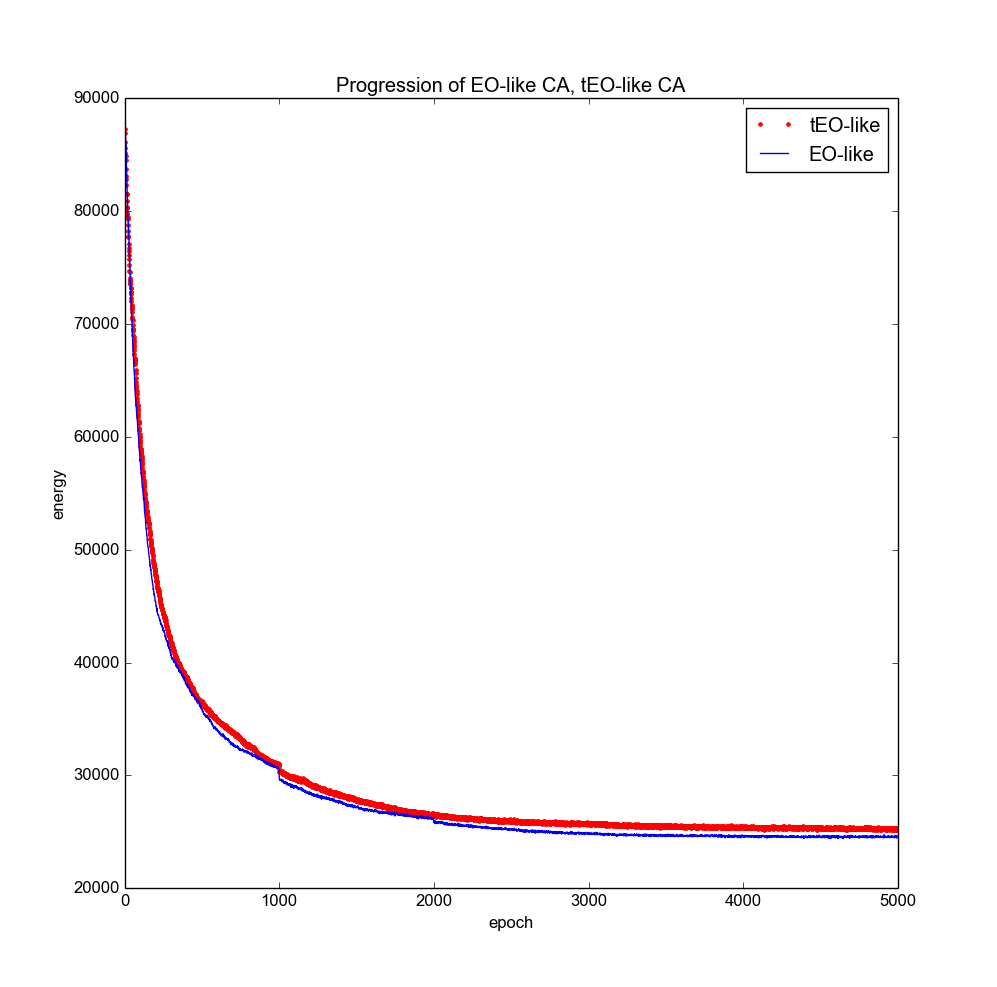
\includegraphics{eo_rbm_unzoomed}
  \end{figure}
 
  \begin{figure}
    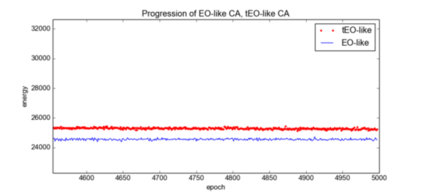
\includegraphics{eo_rbm_zoomed}
  \end{figure}

  Make an algorithm that actually differs from CDiv

  Try non-restricted RBM, and learn with regular gradient

  (using EO in place of SA)

%%%% organization

\section{Stuff} %%%%%

\section{} %What is the issue or question you will be addressing?

\section{} %Why is it interesting, what has previously been done, and what remains to be done?

\section{Novel Approach} %What approach will you be taking to address it? (at a big picture level; novel and/or otherwise noteworthy aspects)

\section{Details of Approach}%Specific target phenomenon or phenomena you will be addressing: e.g., pattern of data you intend to try to fit. Model network task setting, architecture, processing and learning algorithm, training environment (corpus used for training, knowledge base built in to network),

\section{Results and Analysis}

%%First present your primary findings that bear directly on the target phenomena.

%%A strong paper will, in addition, present an analysis of why the results came out the way they did, especially in cases where results did not come out as expected. 

%%It can be useful to discuss results you obtain with one of us to get suggestions as to how to fully understand your findings.

%%Analysis not only of network outputs but also of the structure of the information present in the materials you use to train your network (when relevant) and / or the hidden unit activations, network weights, or learning trajectory can help illuminate why and how your network has performed the way it did.

\section{Discussion}

%Summarize your goals, your approach, and your main findings, and state a conclusion indicating how well, overall, your goals have been met.

%Then, discuss shortcomings or limitations of your effort and indicate how these might be overcome in future work.

%%Also, indicate broader implications and potential future applications of the ideas and approach.

\section{Summary}

Citations:   We will not be sticklers for details of citation styles but do provide citations to literature you draw on in your paper, using the following format

\end{document}

